\label{sec:03IdentifyARMAmodel}
\section{Identify ARMA model}
Now that our time series is stationary, we can determine values of p and q for our ARMA(p,q) model. Several methods exist to determine them. \\

\subsection{With auto.arima() function built-in R}
There is a built-in function in R which helps to determine values of $p$ and $q$ for an ARMA model. This is a first "automatic" result which will serve to do comparisons with our results. \\
Note that it also gives values of parameter d, and (P,D,Q) parameters for the seasonal part if it exists. \\
We have performed several tests with this function. \\
For example, 
\begin{lstlisting}[language=R]
auto.arima(data,seasonal=FALSE, stepwise=FALSE, approximation=FALSE)
\end{lstlisting}
forced \textit{auto.arima()} to run longer and with more trial/error testing cases, and selected an ARMA(3,2) model. \\
However 
\begin{lstlisting}[language=R]
auto.arima(data,seasonal=FALSE, stepwise=TRUE, approximation=TRUE)
\end{lstlisting} 
returned an ARMA(1,0) model.


\subsection{With extended autocorrelation function (EACF)}

Table 5 shows the sample EACF and Table 4 its corresponding simplified table for the series, obtained via the \textit{TSA} package.
\FloatBarrier
\begin{table}[!htbp]
	\centering
  \begin{tabular}{|l||*{11}{c|}}
  \hline
  \backslashbox{AR}{MA}
  &\makebox[1em]{0}&\makebox[1em]{1}&\makebox[1em]{2}
  &\makebox[1em]{3}&\makebox[1em]{4}&\makebox[1em]{5}
  &\makebox[1em]{6}&\makebox[1em]{7}&\makebox[1em]{8}
  &\makebox[1em]{9}&\makebox[1em]{10} \\
  \hline\hline
  0 &X&X&X&X&X&X&X&X&X&X&X\\\hline
  1 &O&O&X&O&X&X&O&O&O&O&O\\\hline
  2 &X&O&O&O&X&X&O&O&O&O&O\\\hline
  3 &X&X&O&O&X&X&O&O&O&O&O\\\hline
  4 &X&X&X&O&O&X&X&X&O&O&O\\\hline
  5 &X&X&X&X&O&X&O&O&O&O&O\\\hline
  6 &X&X&X&X&X&X&O&O&O&O&O\\\hline
  7 &X&X&O&X&X&O&X&O&O&O&O\\\hline
  \end{tabular}
  \caption{Simplified table for EACF}
\end{table}
\FloatBarrier
\FloatBarrier
\begin{table}[!htbp]
	\centering
  \begin{tabular}{|l||*{11}{c|}}
  \hline
  \backslashbox{AR}{MA}
  &\makebox[1em]{0}&\makebox[1em]{1}&\makebox[1em]{2}
  &\makebox[1em]{3}&\makebox[1em]{4}&\makebox[1em]{5}
  &\makebox[1em]{6}&\makebox[1em]{7} \\
  \hline\hline
0 & 0.960 & 0.9227 & 0.8884 & 0.8519 & 0.820 & 0.797 & 7.7e-01 & 0.7403 \\\hline
1 & -0.028 &-0.0150 & 0.0568 &-0.0438 &-0.099 &0.069 & 2.6e-02 & 0.0186  \\\hline
2& -0.426& -0.0087&  0.0288& -0.0277& -0.091 &0.091 &-1.5e-02& -0.0065  \\\hline
3&  0.260 & 0.3307 &-0.0052 &-0.0186 &-0.060& 0.094& -2.0e-02 &-0.0151 \\\hline
4 & 0.477 & 0.2467 &-0.2051& -0.0061& -0.046& 0.079 & 7.1e-02 & 0.0732 \\\hline
5 &-0.350 & 0.4322& -0.3204&  0.1046&-0.033& 0.081 &-1.7e-04 & 0.0342 \\\hline
6&  0.440&  0.3787&  0.3165&  0.3120  &0.244& 0.081 &-5.6e-05& 0.0269 \\\hline
7 &-0.419& -0.0716 &-0.0093&  0.1480 &-0.101& 0.010 &7.7e-02&  0.0304 \\\hline
  \end{tabular}
  \caption{EACF table}
\end{table}
\FloatBarrier

The simplified  table 4 exhibits  a  triangular  pattern  of  “O”  with  its  upper  left  vertex  at  the  order  (p,q) = (1,0).
A few exceptions of “X” appear when q = 2, 4, 5, 6 and 7.
However, the EACF table  shows  that  the  values  of  sample  ACF  corresponding  to  those  “X”  are  around 0.08 or 0.09.
These ACFs are only slightly greater than $2 / \sqrt{1280} = 0.0559$. Indeed, if 3\% critical value is used, those “X” would become “O” in the simplified EACF table.
Consequently,  the  EACF  suggests  that  the  time series  follows an ARMA(1,0) model.


\subsection{With information criteria AIC \& BIC}

\subsubsection{Selection rule}
To use AIC to select an ARMA model in practice, one computes $AIC(i,j)$ for $i = 0,...,P$, $j = 0,...,Q$, where $P$ and $Q$ are prespecified positive integers and selects the orders $(p,q)$ that has the minimum AIC value.
\\
The same rule applies to BIC.
\\

\subsubsection{Results}
For our analysis, we obtain the following tables for AIC and BIC values.

AIC has a minimum value of -7979.095 for (p,q) = (7,7), and so would prefer an ARMA(7,7) model, whereas BIC would select an ARMA(1,0) model since it reaches its minimum value of -7940.592 for (p,q) = (1,0) \\

\underline{Remark:} We can notice that the value of AIC(3,2) is a local minimum in Table 5, and ARMA(3,2) was a potential candidate from \textit{auto.arima()} function. Therefore, this model could be a compromise, since it has a better AIC than ARMA(1,0) and less parameters than ARMA(7,7). \\

\FloatBarrier
\begin{table}[!htbp]
  \centering
  \begin{tabular}{|l||*{10}{c|}}\hline
\backslashbox{p}{q}
&\makebox[3em]{0}&\makebox[3em]{1}&\makebox[3em]{2}
&\makebox[3em]{3}&\makebox[3em]{4}&\makebox[3em]{5}
&\makebox[3em]{6}\\
\hline\hline
0 &-4663.050&-5956.074&-6675.836&-7041.741&-7375.061&-7509.821&-7595.880\\\hline
1 &-7956.056&-7955.018&-7953.200&-7954.187&-7955.289&-7963.993&-7967.363\\\hline
2 &-7955.005&-7953.072&-7952.094&-7952.759&-7951.573&-7965.143&-7967.512\\\hline
3 &-7953.304&-7952.396&-7961.873&-7961.244&-7959.894&-7964.671&-7965.805\\\hline
4 &-7955.051&-7953.458&-7961.332&-7959.371&-7960.121&-7962.767&-7960.667\\\hline
5 &-7955.061&-7952.697&-7959.003&-7959.599&-7972.342&-7971.264&-7973.164\\\hline
6 &-7965.151&-7965.741&-7964.712&-7963.150&-7971.495&-7970.143&-7968.482\\\hline
7 &-7967.376&-7968.029&-7966.036&-7964.594&-7971.115&-7975.143&-7967.147\\\hline
8 &-7966.607&-7966.032&-7964.029&-7969.871&-7971.906&-7969.088&-7967.039\\\hline
9 &-7965.696&-7964.296&-7978.027&-7974.690&-7964.050&-7968.126&-7979.055\\\hline
\end{tabular}
\caption{Table with AIC values (first part)}
\end{table}

\FloatBarrier
\begin{table}[!htbp]
  \centering
  \begin{tabular}{|l||*{10}{c|}}\hline
\backslashbox{p}{q}
&\makebox[3em]{7}&\makebox[3em]{8}&\makebox[3em]{9}\\
\hline\hline
0 &-7672.402&-7712.736&-7761.958\\\hline
1 &-7966.806&-7965.549&-7964.442\\\hline
2 &-7965.795&-7963.914&-7962.569\\\hline
3 &-7965.519&-7963.101&-7962.896\\\hline
4 &-7961.823&-7959.993&-7968.672\\\hline
5 &-7972.918&-7971.996&-7955.056\\\hline
6 &-7968.623&-7960.931&-7960.527\\\hline
7 &-7979.095&-7977.973&-7952.614\\\hline
8 &-7960.482&-7962.310&-7960.790\\\hline
9 &-7955.190&-7968.666&-7964.813\\\hline
\end{tabular}
\caption{Table with AIC values (second part)}
\end{table}

\FloatBarrier
\begin{table}[!htbp]
\centering
\begin{tabular}{|l||*{8}{c|}}\hline
\backslashbox{p}{q}
&\makebox[3em]{0}&\makebox[3em]{1}&\makebox[3em]{2}
&\makebox[3em]{3}&\makebox[3em]{4}&\makebox[3em]{5}
&\makebox[3em]{6}&\makebox[3em]{7} \\ 
\hline\hline
0 &-4652.740&-5940.610&-6655.217&-7015.968&-7344.134&-7473.738&-7554.643&-7626.010\\\hline
1 &-7940.5920&-7934.400&-7927.426&-7923.260&-7919.206&-7922.756&-7920.971&-7915.260\\\hline
2 &-7934.387&-7927.299&-7921.167&-7916.676&-7910.336&-7918.752&-7915.965&-7909.095\\\hline
3 &-7927.531&-7921.468&-7925.790&-7920.007&-7913.503&-7913.125&-7909.104&-7903.663\\\hline
4 &-7924.124&-7917.376&-7920.095&-7912.980&-7908.575&-7906.066&-7898.811&-7894.813\\\hline
5 &-7918.979&-7911.460&-7912.611&-7908.053&-7915.641&-7909.408&-7906.154&-7900.753\\\hline
6 &-7923.914&-7919.350&-7913.166&-7906.449&-7909.640&-7903.133&-7896.318&-7891.304\\\hline
7 &-7920.985&-7916.483&-7909.335&-7902.738&-7904.105&-7902.978&-7889.828&-7896.621\\\hline
\end{tabular}
\caption{Table with BIC values}
\end{table}
\FloatBarrier
This example shows that different approaches or criteria to order determination may result in different choices of $p$ and $q$. There is no evidence to suggest that one method outperforms the other in a real application. Substantive information of the problem under study and simplicity are two factors that also play an important role in choosing an ARMA model for a given time series.

\subsection{With ACF and PACF}

\FloatBarrier
\begin{figure}[!htbp]
  \centering
  \includegraphics[width=\textwidth]{img/Fig7d.eps}
  \caption{ACF of the Random Part of the Serie}
\end{figure}
\FloatBarrier
\begin{figure}[!htbp]
  \centering
  \includegraphics[width=\textwidth]{img/Fig7e.eps}
  \caption{PACF of the Random Part of the Serie}
\end{figure}
\FloatBarrier
We see from the correlogram (Figure 10) that the autocorrelations for many lags in a row exceed the significance bounds, are positive, decrease in magnitude with increasing lag, and tail off to zero after lag 40. Therefore the autocorrelation function shows significant autocorrelation. This does not necessarily mean the series is non-stationary, but it's telling us that the observations are not independent. \\
From the partial autocorrelogram (Figure 11), we see that the partial autocorrelation at lag 1 is positive and exceeds the significance bounds (0.96), while it tails off to zero after lag 1 (with some exceptions for lags 6, 7, and 25, but their excess is very low). Thus an AR(1) model seems possible for the time series.


\subsection{Conclusion}
According to our results, we decided to work with an ARMA(1,0) model, since it is the one selected by EACF method, BIC criterion, and $auto.arima()$ function. Other models that could have been selected are ARMA(7,7) for its best AIC value, or ARMA(3,2) to get a compromise between ARMA(1,0) and ARMA(7,7) as explained above.\\


Therefore, we deduce from the Listing 3, noting our time series $(X_t)$, that
\begin{align*}
X_t−0,0022 
 	&= 0,9621[X_{t-1}−0,0022] + W_t \\
\text{i.e.} \ X_t 
	&= 8,338.10^{-5} + 0,9621 X_{t-1} + W_t
\end{align*}
where $W_t$ is $\mathcal{N}(0,1)$ noise.
\begin{lstlisting}[language=R, caption=ARMA model]
Call:
arima(x = random_stl, order = c(1, 0, 0), seasonal = c(0, 0, 0))

Coefficients:
         ar1  intercept
      0.9621     0.0022
s.e.  0.0076     0.0078

sigma^2 estimated as 0.0001162:  log likelihood = 3981.03,  aic = -7956.06
\end{lstlisting}